\chapter{Diagram algebras}\label{ch:diag}

This chapter provides necessary background on diagram algebras and is modeled after \cite{Ernst2012}.

%%%%%%%%%%%%% Undecorated diagrams %%%%%%%%%%%%%

\begin{section}{Undecorated diagrams}\label{undec}

First, we discuss undecorated diagrams and their corresponding diagram algebras.

\begin{definition}\label{def:k-box}
\rm Let $k$ be a nonnegative integer.  The \emph{standard $k$-box} is a rectangle with $2k$ points, called \emph{nodes},  labeled as in Figure~\ref{Fig073}.  We will refer to the top of the rectangle as the \emph{north face} and the bottom as the \emph{south face}.
\end{definition}


\begin{figure}[!ht]
\centering
\begin{tikzpicture}
\kbox{0};
\draw \foreach \x in {1,2,3} {(\x,0) node[label=above:${\x}$]{}}; 
\draw \foreach \x in {1,2,3} {(\x,-2) node[label=below:${\x}^{\prime}$]{}};
\draw {(5,0) node[label=above:$k$]{}};
\draw {(5,-2) node[label=below:$k^{\prime}$]{}};
\end{tikzpicture}
\caption{The standard $k$-box.}\label{Fig073}
\end{figure}

The next definition summarizes the construction of the ordinary Temperley--Lieb pseudo diagrams.  

\begin{definition}\label{def:T_k(emptyset)}
\rm A \emph{concrete pseudo $k$-diagram} consists of a finite number of disjoint curves (planar), called \emph{edges}, embedded in the standard $k$-box with the following restrictions.  
\begin{enumerate}[leftmargin=0.6in]
\item Every node of the box is the endpoint of exactly one edge, which meets the box transversely. 
\item All other edges must be closed (isotopic to circles) and disjoint from the box. 
\end{enumerate}
\end{definition}


\begin{example}\label{ex:pseudo diagram}
\rm The diagram in Figure~\ref{psuedo} is an example of a concrete pseudo 5-diagram, whereas the diagram in Figure~\ref{fig:notp} does not represent a concrete pseudo 5-diagram since the diagram contains edges that are not disjoint (i.e., they intersect), node $4$ is the endpoint for more than one edge, and node $5$ is not an endpoint for any edge.
\end{example}

\begin{figure}[!h]
\centering
\begin{subfigure}[b]{0.4\textwidth}
\centering
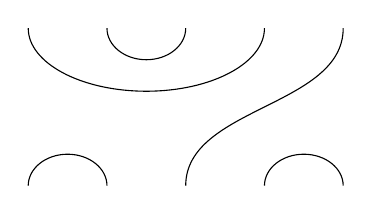
\begin{tikzpicture}
\fivebox{0};
\draw (1,0)  arc (-180:0:1.5 and 0.8) ;
\draw (2,0)  arc (-180:0:0.5 and 0.4) ;
\draw (1,-2)  arc (180:0:0.5 and 0.4) ;
\draw (4,-2)  arc (180:0:0.5 and 0.4) ;
\draw (5,0) .. controls (5,-1) and (3,-1) ..  (3,-2);
\lp{-0.5};
\end{tikzpicture}
\caption{A concrete pseudo 5-diagram}
\label{psuedo}
\end{subfigure}
\quad
\begin{subfigure}[b]{0.4\textwidth}
\centering
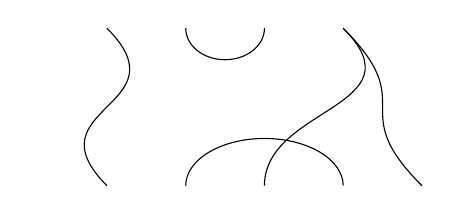
\begin{tikzpicture}
\fivebox{0};
\draw (2,0)  arc (-180:0:0.5 and 0.4) ;
\draw (2,-2)  arc (180:0:1 and 0.6) ;
\draw (1,0) .. controls (2,-1) and (0,-1) .. (1,-2);
\draw (4,0) .. controls (5,-1) and (4,-1) .. (5,-2);
\draw (4,0) .. controls (5,-1) and (3,-1) .. (3,-2);
\end{tikzpicture}
\caption{Not a concrete pseudo 5-diagram}
\label{fig:notp}
\end{subfigure}
\caption{Examples of diagrams.}
\end{figure}

 We now define an equivalence relation on the set of concrete pseudo $k$-diagrams. Two concrete pseudo $k$-diagrams are \emph{(isotopically) equivalent} if one concrete diagram can be obtained from the other by isotopically deforming the edges such that any intermediate diagram is also a concrete pseudo $k$-diagram. Note that an isotopy of the k-box is a 1-parameter family of homeomorphisms of the $k$-box to itself that are stationary on the boundary.
\begin{definition}
A \emph{pseudo $k$-diagram} (or an \emph{ordinary Temperley--Lieb pseudo-diagram}) is defined to be an equivalence class of equivalent concrete pseudo $k$-diagrams.  We denote the set of pseudo $k$-diagrams by $T_{k}(\emptyset)$.
\end{definition}

\begin{remark}\label{vertequiv}
When representing a pseudo $k$-diagram with a drawing, we pick an arbitrary concrete representative among a continuum of equivalent choices. When no confusion can arise, we will not make a distinction between a concrete pseudo $k$-diagram and the equivalence class that it represents. We say that two concrete pseudo $k$-diagrams are \emph{vertically equivalent} if they are equivalent in the above sense by an isotopy that preserves setwise each vertical cross-section of the $k$-box.
\end{remark}

\begin{example}
The concrete pseudo $5$-diagram in Figure~\ref{psuedo} and the concrete pseudo $5$-diagram in Figure~\ref{equivpseudo} are equivalent concrete pseudo $5$-diagrams since the diagram in Figure~\ref{psuedo} can be obtained by isotopically deforming the edges in Figure~\ref{equivpseudo}.

\begin{figure}[!h]
\centering
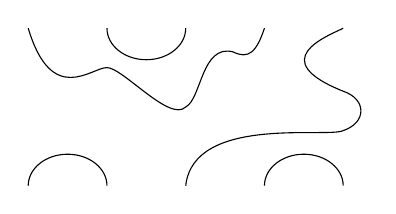
\begin{tikzpicture}
\fivebox{0};
\draw (1,0)  .. controls (1.3,-1) and (1.8,-0.5)  .. (2,-0.5) .. controls (2.2,-0.5) and (2.8,-1.2) .. (3,-1) .. controls (3.2,-0.9) and (3.2,-0.2) .. (3.6,-0.3) .. controls (3.8,-0.4) and (3.9,-0.3) .. (4,0);
\draw (2,0)  arc (-180:0:0.5 and 0.4) ;
\draw (1,-2)  arc (180:0:0.5 and 0.4) ;
\draw (4,-2)  arc (180:0:0.5 and 0.4) ;
\draw (5,0) .. controls (4.8,-0.1) and (4,-0.4) .. (5,-0.8) .. controls (5.3,-0.9) and (5.3,-1.2) .. (5,-1.3) .. controls (4.8,-1.4) and (3.1,-1.1) .. (3,-2);
\lp{-0.5};
\end{tikzpicture}
%\caption{Isotopic deformation of a diagram.}
\caption{An isotopically equivalent diagram of Figure~\ref{psuedo}.}
\label{equivpseudo}
\end{figure}
\end{example}

Let $d$ be a diagram and let $e$ be an edge of $d$. If $e$ is a closed curve occurring in $d$, then we call $e$ a \emph{loop}.  For example, the diagram in Figure~\ref{psuedo} has a single loop.  If $e$ joins node $i$ in the north face to node $j'$ in the south face, then $e$ is called a \emph{propagating edge from $i$ to $j'$}. If $e$ is not propagating, loop or otherwise, it will be called \emph{non-propagating}.  
%If a propagating edge joins $i$ to $i'$, then we will call it a \emph{vertical propagating edge}.  

Note that we used the word ``pseudo'' in our definition to emphasize that we allow loops to appear in our diagrams. In Section \ref{decorated}, we will add decorations to our diagrams. The presence of $\emptyset$ in the definition above is to emphasize that the edges of the diagrams are undecorated.


Note that the number of non-propagating edges in the north face of a diagram must be equal to the number of non-propagating edges in the south face.  We define the function $\a: T_{k}(\emptyset) \to \Z^{+}\cup \{0\}$ via
\[
\a(d)=\text{ number of non-propagating edges in the north face of } d
\]
and the function $\mathbf{p}: T_{k}(\emptyset) \to \Z^{+}\cup \{0\}$ via
\[
\mathbf{p}(d)=\text{ number of propagating edges in the north face of } d
\]
where $2\a(d)+\mathbf{p}(d)=k$.
For example, Figure~\ref{psuedo} has two non-propagating edges and one propagating edge in the north face and therefore, $\a(d)=2$ and $\mathbf{p}(d)=1$. There is only one diagram with $\a$-value $0$ having no loops; namely the diagram $d_{e}$ that appears in Figure~\ref{Fig076}.  The maximum value that $\a(d)$ can take is $\lfloor k/2 \rfloor$.  

\begin{figure}[!ht]
\centering
$d_{e}:=$
\begin{tabular}[c]{l}
\begin{tikzpicture}
\kbox{0}
\draw (1,0) -- (1,-2);
\draw (2,0) -- (2,-2);
\draw (3,0) -- (3,-2);
\node at (4,-1) {$\cdots$};
\draw (5,0) -- (5,-2);
\end{tikzpicture}
\end{tabular}
\caption{The only diagram having $\a$-value 0 and no loops.}\label{Fig076}
\end{figure}


We wish to define an associative algebra that has the pseudo $k$-diagrams as a basis.

\begin{definition}\label{def:P_k(emptyset)}
\rm Let $R$ be a commutative ring with $1$.  The associative algebra $\P_{k}(\emptyset)$ over $R$ is the free $R$-module having $T_{k}(\emptyset)$ as a basis, with multiplication (referred to as diagram concatenation) defined as follows. We define multiplication in $\P_{k}(\emptyset)$ by defining multiplication in the case where $d$ and $d'$ are basis elements, and then extend bilinearly. If $d, d' \in T_{k}(\emptyset)$, the product $d'd$ is the element of $T_{k}(\emptyset)$ obtained by placing $d'$ on top of $d$, so that node $i'$ of $d'$ coincides with node $i$ of $d$. %rescaling vertically by a factor of $1/2$ to recover a standard $k$-box. 
\end{definition}

\begin{example}\label{looploop}
Figure~\ref{Fig:looploop} depicts the product of three basis diagrams from $\P_{5}(\emptyset)$.

\begin{figure}[!ht]
\centering
$\begin{tabular}[c]{l}
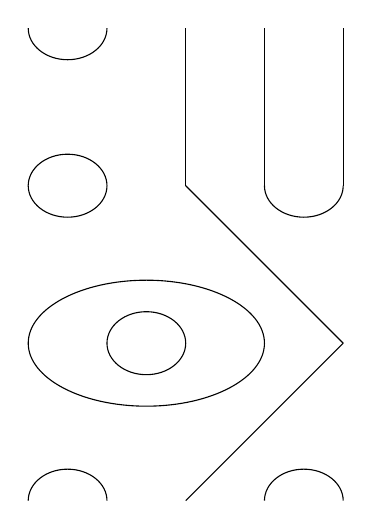
\begin{tikzpicture}
\fivebox{0};
\draw (1,0)  arc (-180:0:1.5 and 0.8) ;
\draw (2,0)  arc (-180:0:0.5 and 0.4) ;
\draw (1,-2)  arc (180:0:0.5 and 0.4) ;
\draw (4,-2)  arc (180:0:0.5 and 0.4) ;
\draw (5,0) -- (3,-2);
\fivebox{2};
\draw (1,0)  arc (180:0:1.5 and 0.8) ;
\draw (2,0)  arc (180:0:0.5 and 0.4) ;
\draw (1,2)  arc (-180:0:0.5 and 0.4) ;
\draw (4,2)  arc (-180:0:0.5 and 0.4) ;
\draw (5,0) -- (3,2);
\fivebox{4};
\draw (1,4)  arc (-180:0:0.5 and 0.4) ;
\draw (1,2)  arc (180:0:0.5 and 0.4) ;
\draw (3,4) -- (3,2);
\draw (4,4) -- (4,2);
\draw (5,4) -- (5,2);
\end{tikzpicture}
\end{tabular}
=  
\ \begin{tabular}[c]{l}
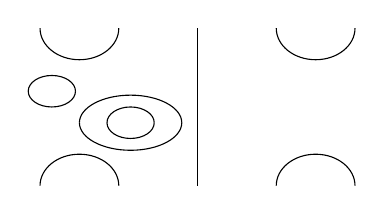
\begin{tikzpicture}
\fivebox{0};
\draw (0.85,-0.8) arc(-180:0:0.3 and 0.2);
\draw (0.85,-0.8) arc(180:0:0.3 and 0.2);
\draw (1.85,-1.2) arc(-180:0:0.3 and 0.2);
\draw (1.85,-1.2) arc(180:0:0.3 and 0.2);
\draw (1.5,-1.2) arc(-180:0:0.65 and 0.35);
\draw (1.5,-1.2) arc(180:0:0.65 and 0.35);
\draw (1,0)  arc (-180:0:0.5 and 0.4) ;
\draw (1,-2)  arc (180:0:0.5 and 0.4) ;
\draw (4,0)  arc (-180:0:0.5 and 0.4) ;
\draw (4,-2)  arc (180:0:0.5 and 0.4) ;
\draw (3,0) -- (3,-2);
\end{tikzpicture}
\end{tabular}$
\caption{An example of multiplication in $\P_{5}(\emptyset)$.}\label{Fig:looploop}
\end{figure}
\end{example}

We now restrict our attention to a particular base ring, namely, let $R=\Z[\delta]$, the ring of polynomials in $\delta$ with integer coefficients.
\begin{definition}\label{def:DTL(A_n)}
\rm Let $\DTL(A_{n})$ be the associative $\Z[\delta]$-algebra equal to the quotient of $\P_{n+1}(\emptyset)$ determined by the relation depicted in Figure~\ref{Fig077}.
\end{definition}

\begin{figure}[!ht]
\centering
\begin{tabular}[c]{@{} c@{}}
\begin{tikzpicture}
\lp{0};
\end{tikzpicture}
\end{tabular}
$= \delta$
\caption{The defining relation of $\DTL(A_{n})$.}\label{Fig077}
\end{figure}

It is well-known that $\DTL(A_{n})$ is the free $\Z[\delta]$-module with basis given by the elements of $T_{n+1}(\emptyset)$ having no loops. The multiplication is inherited from the multiplication on $\P_{n+1}(\emptyset)$ except we multiply by a factor of $\delta$ for each resulting loop and then discard the loop.  We will refer to $\DTL(A_{n})$ as the \emph{ordinary Temperley--Lieb diagram algebra}.

\begin{example}
\rm Figure~\ref{Fig078--Fig079} depicts the product of three basis diagrams from $\DTL(A_{4})$. Note that this is the same product of diagrams as in Example~\ref{looploop}, however, in this case the three loops are replaced with the coefficient $\delta^3$.

\begin{figure}[!ht]
\centering
$\begin{tabular}[c]{l}
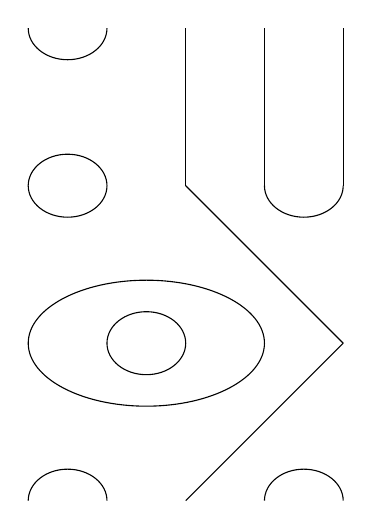
\begin{tikzpicture}
\fivebox{0};
\draw (1,0)  arc (-180:0:1.5 and 0.8) ;
\draw (2,0)  arc (-180:0:0.5 and 0.4) ;
\draw (1,-2)  arc (180:0:0.5 and 0.4) ;
\draw (4,-2)  arc (180:0:0.5 and 0.4) ;
\draw (5,0) -- (3,-2);
\fivebox{2};
\draw (1,0)  arc (180:0:1.5 and 0.8) ;
\draw (2,0)  arc (180:0:0.5 and 0.4) ;
\draw (1,2)  arc (-180:0:0.5 and 0.4) ;
\draw (4,2)  arc (-180:0:0.5 and 0.4) ;
\draw (5,0) -- (3,2);
\fivebox{4};
\draw (1,4)  arc (-180:0:0.5 and 0.4) ;
\draw (1,2)  arc (180:0:0.5 and 0.4) ;
\draw (3,4) -- (3,2);
\draw (4,4) -- (4,2);
\draw (5,4) -- (5,2);
\end{tikzpicture}
\end{tabular}
= \  \delta^{3} \ \begin{tabular}[c]{l}
\begin{tikzpicture}
\fivebox{0};
\draw (1,0)  arc (-180:0:0.5 and 0.4) ;
\draw (1,-2)  arc (180:0:0.5 and 0.4) ;
\draw (4,0)  arc (-180:0:0.5 and 0.4) ;
\draw (4,-2)  arc (180:0:0.5 and 0.4) ;
\draw (3,0) -- (3,-2);
\end{tikzpicture}
\end{tabular}$
\caption{An example of multiplication in $\DTL(A_{4})$.}\label{Fig078--Fig079}
\end{figure}
\end{example}

The next theorem describes the connection between $\TL(A_n)$ and $\DTL(A_n)$ shown in \cite{Kauffman1987} and \cite{Penrose1971}.

\begin{theorem}\label{kauff}
{\rm (Kaufmann, \cite{Kauffman1987})}
As $\Z[\delta]$-algebras, the Temperley--Lieb algebra $\TL(A_{n})$ is isomorphic to $\DTL(A_{n})$.  Moreover, each loop-free diagram from $T_{n+1}(\emptyset)$ corresponds to a unique monomial basis element of $\TL(A_{n})$.  
\qed
\end{theorem}

\end{section}

%%%%%%%%%%%%% Decorated diagrams %%%%%%%%%%%%%

\begin{section}{Decorated diagrams}\label{decorated}
We now describe the construction of diagrams whose edges carry decorations. We will use the symbol $\bcirc$, which we refer to as a \emph{decoration}, to adorn the edges of a diagram. Let $\mathbf{b}=x_{1}x_{2}\cdots x_{r}$ be a finite sequence of decorations, where each $x_i=\bcirc$. We say that $\mathbf{b}$ is a \emph{block} of decorations of \emph{width} $r$.  Note that a block of width $1$ is just a single decoration.  The string $\bcirc~\bcirc~\bcirc~\bcirc~\bcirc~\bcirc~\bcirc$ is an example of a block of width 7.

Ultimately, we have three restrictions (D0, D1, D2) for how we allow the edges of a diagram to be decorated by blocks, which we will now outline. Note that we are maintaining consistency with cases involving multiple decoration types as in \cite{Ernst2012}, and that $\a(d)$ is defined the same way as in type $A_n$. Let $d$ be a fixed concrete pseudo $k$-diagram and let $e$ be an edge of $d$.

\begin{enumerate}[leftmargin=0.6in]

\item[(D0)] If $\a(d)=0$, then $e$ is undecorated.

\end{enumerate}

\noindent In particular, the unique diagram $d_{e}$ with $\a$-value 0 and no loops is undecorated.
Subject to some restrictions, if $\a(d)>0$, we may adorn $e$ with a finite sequence of blocks of decorations $\mathbf{b}_{1}, \dots, \mathbf{b}_{m}$ such that adjacency of blocks and decorations of each block is preserved as we travel along $e$.  

If $e$ is a non-loop edge, the convention we adopt is that the decorations of the block are placed so that we can read off the sequence of decorations as we traverse $e$ from $i$ to $j'$ if $e$ is propagating, or from $i$ to $j$ (respectively, $i'$ to $j'$) with $i < j$ (respectively, $i' < j'$) if $e$ is non-propagating.

If $e$ is a loop, reading the corresponding sequence of decorations depends on an arbitrary choice of starting point and direction round the loop.


If $\a(d)\neq 0$, then we also require the following.

\begin{enumerate}[leftmargin=0.6in]
\item[(D1)] We allow adjacent blocks on $e$ to be conjoined to form larger blocks.


%\item[(D3)] If $\a(d)>1$ and $e$ is propagating, then as in (D2), we allow adjacent blocks on $e$ to be conjoined to form larger blocks.

\end{enumerate}

\begin{definition}
A \emph{concrete decorated pseudo $k$-diagram} is any concrete pseudo $k$-diagram with decorations satisfying (D0) and (D1).
\end{definition}

\begin{definition}
We define two concrete pseudo decorated $k$-diagrams to be equivalent if we can isotopically deform one diagram into the other such that any intermediate diagram is also a concrete decorated pseudo $k$-diagram. 
\end{definition}

\begin{definition}\label{def:T_{k}(Omega)}
\rm A \emph{decorated pseudo $k$-diagram} is defined to be an equivalence class of equivalent concrete decorated pseudo $k$-diagrams.  We denote the set of decorated diagrams by $T_{k}(\bcirc)$.
Then define $\P_{k}(\bcirc)$ to be the free $\Z[\delta]$-module having the decorated pseudo $k$-diagrams $T_{k}(\bcirc)$ as a basis.  
\end{definition}

We define multiplication in $\P_{k}(\bcirc)$ by concatenating diagrams, conjoining blocks and extending bilinearly (as in Definition~\ref{def:P_k(emptyset)}). It follows from Section 3 of \cite{Ernst2012} that the multiplication just defined turns $\P_{k}(\bcirc)$ into a well-defined associative $\Z[\delta]$-algebra.

%defining multiplication (diagram concatenation) in the case where $d$ and $d'$ are basis elements, and then extend bilinearly.  To calculate the product $d'd$, concatenate $d'$ and $d$ While maintaining equivalence, conjoin adjacent blocks. 
 
\begin{example}\label{ex:decorated diagrams}
\rm Here are a few examples.
\begin{enumerate}[leftmargin=0.6in]
\item  The diagram in Figure~\ref{Fig080} is an example of a decorated pseudo $5$-diagram. The decorations on the unique propagating edge can be conjoined to form a maximal block of width 4.

\item  The diagram in Figure~\ref{Fig081} is another example of a decorated pseudo $5$-diagram, but with $\a$-value 1.  Note that the decorations can be conjoined to form a block of width 3.

\item Figure~\ref{fig:product} depicts the product of the diagram in Figure~\ref{Fig080} and the diagram in Figure~\ref{Fig081}.
\end{enumerate}
\end{example}

\begin{figure}[!ht]
\centering
\subcaptionbox{\label{Fig081}}{
\begin{tikzpicture}
\fivebox{0};
\draw (1,0) -- (1,-2)
	node[fill=cyan, pos=0.25, shape=circle, inner sep=1.8pt, minimum size=2pt]{}
	node[fill=cyan,  pos=0.5, shape=circle, inner sep=1.8pt, minimum size=2pt]{}
	node[fill=cyan,  pos=0.75, shape=circle, inner sep=1.8pt, minimum size=2pt]{};
\draw (2,0)  arc (-180:0:0.5 and 0.4) ;
\draw (2,-2)  arc (180:0:0.5 and 0.4) ;
\draw (4,0) -- (4,-2);
\draw (5,0) -- (5,-2);
\end{tikzpicture}}
\qquad
\subcaptionbox{\label{Fig080}}{
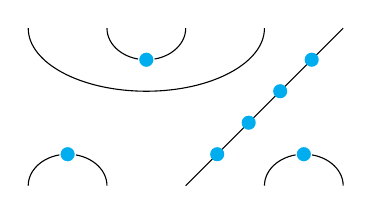
\begin{tikzpicture}
\fivebox{0};
\draw (1,0)  arc (-180:0:1.5 and 0.8) ;
\draw (2,0)  arc (-180:0:0.5 and 0.4) ;
\draw (1,-2)  arc (180:0:0.5 and 0.4) ;
\draw (4,-2)  arc (180:0:0.5 and 0.4) ;
\draw (5,0) -- (3,-2)
	node[fill=cyan,  pos=0.2, shape=circle, inner sep=1.8pt, minimum size=2pt]{}
	node[fill=cyan,  pos=0.4, shape=circle, inner sep=1.8pt, minimum size=2pt]{}
	node[fill=cyan,  pos=0.6, shape=circle, inner sep=1.8pt, minimum size=2pt]{}
	node[fill=cyan,  pos=0.8, shape=circle, inner sep=1.8pt, minimum size=2pt]{}; 
\draw[fill=cyan, draw=white]{(1.5,-1.6) circle (2.8pt)};
\draw[fill=cyan, draw=white]{(2.5,-0.4) circle (2.8pt)};
\draw[fill=cyan, draw=white]{(4.5,-1.6) circle (2.8pt)};
\end{tikzpicture}}
\caption{Examples of decorated pseudo diagrams.}
\end{figure}


\begin{figure}[!ht]
\centering
\begin{tabular}[c]{l}
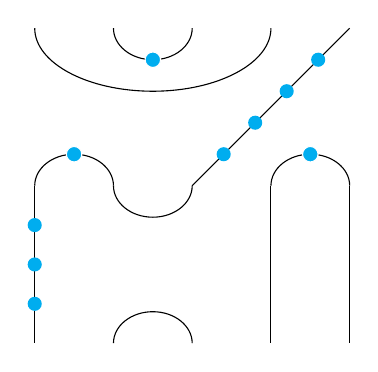
\begin{tikzpicture}
\fivebox{0};
\draw (1,0)  arc (-180:0:1.5 and 0.8) ;
\draw (2,0)  arc (-180:0:0.5 and 0.4) ;
\draw (1,-2)  arc (180:0:0.5 and 0.4) ;
\draw (4,-2)  arc (180:0:0.5 and 0.4) ;
\draw (5,0) -- (3,-2)
	node[fill=cyan,  pos=0.2, shape=circle, inner sep=1.8pt, minimum size=2pt]{}
	node[fill=cyan,  pos=0.4, shape=circle, inner sep=1.8pt, minimum size=2pt]{}
	node[fill=cyan,  pos=0.6, shape=circle, inner sep=1.8pt, minimum size=2pt]{}
	node[fill=cyan,  pos=0.8, shape=circle, inner sep=1.8pt, minimum size=2pt]{};
\draw[fill=cyan, draw=white]{(1.5,-1.6) circle (2.8pt)};
\draw[fill=cyan, draw=white]{(2.5,-0.4) circle (2.8pt)};
\draw[fill=cyan, draw=white]{(4.5,-1.6) circle (2.8pt)};
\fivebox{-2};
\draw (1,-2) -- (1,-4)
	node[fill=cyan,  pos=0.25, shape=circle, inner sep=1.8pt, minimum size=2pt]{}
	node[fill=cyan,  pos=0.5, shape=circle, inner sep=1.8pt, minimum size=2pt]{}
	node[fill=cyan,  pos=0.75, shape=circle, inner sep=1.8pt, minimum size=2pt]{};
\draw (2,-2)  arc (-180:0:0.5 and 0.4) ;
\draw (2,-4)  arc (180:0:0.5 and 0.4) ;
\draw (4,-2) -- (4,-4);
\draw (5,-2) -- (5,-4);
\end{tikzpicture}
\end{tabular}
~$=$~
\begin{tabular}[c]{l}
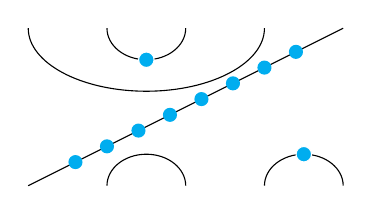
\begin{tikzpicture}
\fivebox{0};
\draw (1,0)  arc (-180:0:1.5 and 0.8) ;
\draw (2,0)  arc (-180:0:0.5 and 0.4) ;
\draw (5,0) -- (1,-2)
	node[fill=cyan,  pos=0.15, shape=circle, inner sep=1.8pt, minimum size=2pt]{}
	node[fill=cyan,  pos=0.25, shape=circle, inner sep=1.8pt, minimum size=2pt]{}
	node[fill=cyan,  pos=0.35, shape=circle, inner sep=1.8pt, minimum size=2pt]{}
	node[fill=cyan,  pos=0.45, shape=circle, inner sep=1.8pt, minimum size=2pt]{}
	node[fill=cyan,  pos=0.55, shape=circle, inner sep=1.8pt, minimum size=2pt]{}
	node[fill=cyan,  pos=0.65, shape=circle, inner sep=1.8pt, minimum size=2pt]{}
	node[fill=cyan,  pos=0.75, shape=circle, inner sep=1.8pt, minimum size=2pt]{}
	node[fill=cyan,  pos=0.85, shape=circle, inner sep=1.8pt, minimum size=2pt]{}; 
\draw (2,-2)  arc (180:0:0.5 and 0.4) ;
\draw (4,-2)  arc (180:0:0.5 and 0.4) ;
\draw[fill=cyan, draw=white]{(2.5,-0.4) circle (2.8pt)};
\draw[fill=cyan, draw=white]{(4.5,-1.6) circle (2.8pt)};
\end{tikzpicture}
\end{tabular}
\caption{The product of two decorated pseudo diagrams}
\label{fig:product}
\end{figure}



In type $D_n$, we also require the decorations to be ``left exposed" (requirement (D2)), a concept that appears in the context of the Temperley--Lieb algebra of type $B$ \cite{Green1998a}.

\begin{enumerate}[leftmargin=0.6in]
\item[(D2)]  All decorated edges can be simultaneously deformed so as to take decorations to the left wall of the diagram without crossing any other edges.
\end{enumerate}

\begin{remark}
In type $D_n$ we only need the decorations to be left-exposed, but some types also require the decorations to be right-exposed---for example, the diagrammatic representation of type $\C_n$ in \cite{Ernst2012}.
\end{remark}

\begin{definition}
\rm A \emph{concrete L-decorated pseudo $k$-diagram} is any concrete decorated pseudo $k$-diagram that also satisfies condition (D2).
\end{definition}

\begin{definition}\label{def:T_{k}^{LR}(Omega)}
\rm An \emph{L-decorated pseudo $k$-diagram} is defined to be an equivalence class of equivalent concrete L-decorated pseudo $k$-diagrams.  We denote the set of equivalence classes from $T_{k}(\bcirc)$ where representatives are concrete L-decorated pseudo $k$-diagrams by $T_{k}^L(\bcirc)$. Then define $\P_{k}^L(\bcirc)$ to be the subalgrebra of $\P_{k}(\bcirc)$ with $T_{k}^L(\bcirc)$ as a basis.  
\end{definition}

Note that ``L" stands for ``left" in the definitions above.
\begin{example}
The diagram in Figure~\ref{Fig081} is an L-decorated diagram, however, the diagram in Figure~\ref{Fig080} is not an L-decorated diagram since there are two edges with decorations that cannot be deformed so as to take the decoration to the left wall of the diagram without crossing another edge.
\end{example}
\begin{remark}
We observe that the product of two L-decorated pseudo $k$-diagrams is a L-decorated pseudo $k$-diagram.
\end{remark}





  %To justify this claim we require the following lemma.

%\begin{lemma}\label{lem:a-value=1}
%{\rm (Ernst,\cite{Ernst2012})} Let $d$ be diagram with $\a(d)=1$.  Suppose that the unique non-propagating edge in the north face %of $d$ joins $i$ to $i+1$.  Let $d'$ be any other diagram with $\a(d')>0$.  Then $\a(d'd)=1$ if and only if $\a(d')=1$ and the unique %non-propagating edge in the south face of $d'$ joins either (a) $(i-1)'$ to $i'$, (b) $i'$ to $(i+1)'$, or (c) $(i+1)'$ to $(i+2)'$.
%\qed
%\end{lemma}

 

\end{section}

%%%%%%%%%%%%% Diagrammatic relations %%%%%%%%%%%%%

\begin{section}{Diagrammatic relations}

Our immediate goal is to define a quotient of $\P_{k}^{L}(\bcirc)$ having relations that are determined by applying local combinatorial rules to the diagrams. 

\begin{definition}\label{def:big diagram alg}
Let $\widehat{\P}_{k}^{L}(\bcirc)$ be the associative $\Z[\delta]$-algebra equal to the quotient of $\P_{k}^{L}(\bcirc)$ by the relations depicted in Figure~\ref{fig:relations}, where the decorations on the edges represent adjacent decorations of the same block.
\end{definition}

\begin{figure}[!ht]
\centering
$\begin{tabular}[c]{l}
\begin{tikzpicture}
\lp{0};
\end{tikzpicture}
\end{tabular}
~$=$~
$\begin{tabular}[c]{l}
\begin{tikzpicture}
\node at (-1.2,0) {};
\node at (-1,0) {$\delta$};
\node at (-0.5,0) {};
\end{tikzpicture}
\end{tabular}
\quad \quad \quad
\begin{tabular}[c]{l}
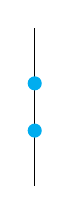
\begin{tikzpicture}
\draw (1,0) -- (1,-2)
	node[fill=cyan,  pos=0.35, shape=circle, inner sep=1.8pt, minimum size=2pt]{}
	node[fill=cyan,  pos=0.65, shape=circle, inner sep=1.8pt, minimum size=2pt]{};
\end{tikzpicture}
\end{tabular}
~$=$~
\begin{tabular}[c]{l}
\begin{tikzpicture}
\draw (1,0) -- (1,-2);
\end{tikzpicture}
\end{tabular}
\quad \quad \quad
$\begin{tabular}[c]{l}
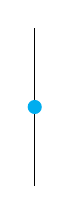
\begin{tikzpicture}
\dlp{0}{-1};
\draw (1,0) -- (1,-2)
	node[fill=cyan,  pos=0.5, shape=circle, inner sep=1.8pt, minimum size=2pt]{};
\end{tikzpicture}
\end{tabular}
~$=$~
$\begin{tabular}[c]{l}
\begin{tikzpicture}
\dlp{0}{-1};
\draw (1,0) -- (1,-2);
\end{tikzpicture}
\end{tabular}
\caption{Defining relations of $\widehat{\P}_{k}^{L}(\bcirc)$.}
\label{fig:relations}
\end{figure}

The third relation in Figure~\ref{fig:relations} means that any edge loses its decortation in the presence of a decorated loop. Using the first and third relation, if there is more than one decorated loop, then all loops are replaced with the coefficient $\delta$ except for one decorated loop. The second relation ensures that no edge may carry more than one decoration. Note that all of the relations are local in the sense that a single reduction involves edges bounding the same region of the diagram. 

\begin{remark}\label{diagbasis}
The local diagrammatic relations for $\P^{L}_{k}(\bcirc)$ make it clear that L-decorated diagrams with no undecorated loops having either exactly one decorated loop and no other decorations or no decorated loops with edges having at most one decoration form a basis for $\P^{L}_{k}(\bcirc)$.
\end{remark}

\begin{example}
Figure~\ref{fig:apply} depicts the relations from Figure~\ref{fig:relations} applied to the diagram from $\P^{L}_{5}(\bcirc)$ in Figure~\ref{Fig081}.
\end{example}

\begin{figure}[!h]
\centering
\begin{tikzpicture}[scale=1]
\fivebox{0};
\draw (1,0) -- (1,-2)
	node[fill=cyan,  pos=0.5, shape=circle, inner sep=1.8pt, minimum size=2pt]{};
\draw (2,0)  arc (-180:0:0.5 and 0.4) ;
\draw (2,-2)  arc (180:0:0.5 and 0.4) ;
\draw (4,0) -- (4,-2);
\draw (5,0) -- (5,-2);
\end{tikzpicture}
\caption{Example of a diagram from $\widehat{\P}_{5}^{L}(\bcirc)$.}
\label{fig:apply}
\end{figure}


\begin{example}
\rm Figure~\ref{Fig101--Fig102} depicts multiplication of three diagrams from $\widehat{\P}_{5}^{L}(\bcirc)$ and Figure~\ref{Fig103--Fig104} shows an example where a decorated loop is present. 
\end{example}

\begin{figure}[!ht]
\centering
\begin{tabular}[c]{l}
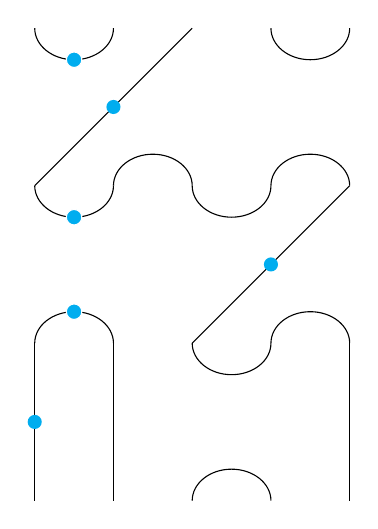
\begin{tikzpicture}[scale=1]
\fivebox{2};
\draw (1,2) arc (-180:0:0.5 and 0.4);
\draw[fill=cyan, draw=white]{(1.5,1.6) circle (2.8pt)};
\draw (3,2) -- (1,0)
	node[fill=cyan,  pos=0.5, shape=circle, inner sep=1.8pt, minimum size=2pt]{};
\draw (2,0) arc (180:0:0.5 and 0.4);
\draw (4,0) arc (180:0:0.5 and 0.4);
\draw (4,2) arc (-180:0:0.5 and 0.4);
\fivebox{0};
\draw (1,0)  arc (-180:0:0.5 and 0.4) ;
\draw (3,0)  arc (-180:0:0.5 and 0.4) ;
\draw (1,-2)  arc (180:0:0.5 and 0.4) ;
\draw (4,-2)  arc (180:0:0.5 and 0.4) ;
\draw (5,0) -- (3,-2)
	node[fill=cyan,  pos=0.5, shape=circle, inner sep=1.8pt, minimum size=2pt]{};
\draw[fill=cyan, draw=white]{(1.5,-1.6) circle (2.8pt)};
\draw[fill=cyan, draw=white]{(1.5,-0.4) circle (2.8pt)};
\fivebox{-2};
\draw (1,-2) -- (1,-4)
	node[fill=cyan,  pos=0.5, shape=circle, inner sep=1.8pt, minimum size=2pt]{};
\draw (2,-2) -- (2,-4);
\draw (3,-2) arc (-180:0:0.5 and 0.4);
\draw (3,-4) arc (180:0:0.5 and 0.4);
\draw (5,-2) -- (5,-4);
\end{tikzpicture}
\end{tabular}
~$=$~
\begin{tabular}[c]{l}
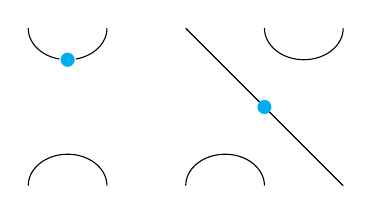
\begin{tikzpicture}[scale=1]
\fivebox{0};
\draw (1,0) arc (-180:0:0.5 and 0.4);
\draw (4,0) arc (-180:0:0.5 and 0.4);
\draw (3,0) -- (5,-2)
	node[fill=cyan,  pos=0.5, shape=circle, inner sep=1.8pt, minimum size=2pt]{};
\draw (1,-2)  arc (180:0:0.5 and 0.4) ;
\draw (3,-2)  arc (180:0:0.5 and 0.4) ;
\draw[fill=cyan, draw=white]{(1.5,-0.4) circle (2.8pt)};
\end{tikzpicture}
\end{tabular}
\caption{Example of multiplication in $\widehat{\P}_{5}^{L}(\bcirc)$.}\label{Fig101--Fig102}
\end{figure} 

\begin{figure}[!ht]
\centering
\begin{tabular}[c]{l}
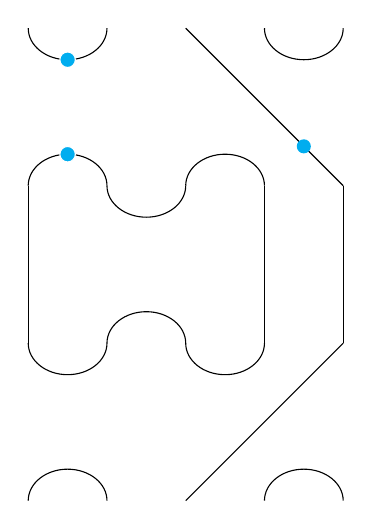
\begin{tikzpicture}[scale=1]
\fivebox{2};
\draw (1,0)  arc (180:0:0.5 and 0.4) ;
\draw[fill=cyan, draw=white]{(1.5,0.4) circle (2.8pt)};
\draw (1,2)  arc (-180:0:0.5 and 0.4) ;
\draw[fill=cyan, draw=white]{(1.5,1.6) circle (2.8pt)};
\draw (3,0)  arc (180:0:0.5 and 0.4) ;
\draw (4,2) arc (-180:0:0.5 and 0.4);
\draw (5,0) -- (3,2)
	node[fill=cyan,  pos=0.25, shape=circle, inner sep=1.8pt, minimum size=2pt]{};
\fivebox{0};
\draw (1,-2) -- (1,0);
\draw (2,0)  arc (-180:0:0.5 and 0.4) ;
\draw (2,-2) arc (180:0:0.5 and 0.4);
\draw (4,0) -- (4,-2);
\draw (5,0) -- (5,-2);
\fivebox{-2};
\draw (1,-2) arc (-180:0:0.5 and 0.4);
\draw (3,-2) arc (-180:0:0.5 and 0.4);
\draw (5,-2) -- (3,-4);
\draw (1,-4) arc (180:0:0.5 and 0.4);
\draw (4,-4) arc (180:0:0.5 and 0.4);
\end{tikzpicture}
\end{tabular}
~$=$~
\begin{tabular}[c]{l}
\begin{tikzpicture}[scale=1]
\fivebox{0};
\draw (1,0) arc (-180:0:0.5 and 0.4);
\draw (4,0) arc (-180:0:0.5 and 0.4);
\draw (3,0) -- (3,-2);
\draw (1,-2)  arc (180:0:0.5 and 0.4) ;
\draw (4,-2)  arc (180:0:0.5 and 0.4) ;
\dlp{1}{-1};
\end{tikzpicture}
\end{tabular}
\caption{Example of multiplication in $\widehat{\P}_{5}^{L}(\bcirc)$ resulting in a decorated loop.}
\label{Fig103--Fig104}
\end{figure}



\end{section}




%%%%%%%%%%%%% Simple diagrams %%%%%%%%%%%%%

\begin{section}{Simple diagrams}\label{sec:simple}
In this section, we define the diagram algebra $\DTL(D_n)$ as a certain subalgebra of $\widehat{\P}_{n+1}^{L}(\bcirc)$ that turns out to be a diagrammatic representation of $\TL(D_n)$. 

Define the \emph{simple diagrams} $d_{\overline{1}}, d_{1}, d_{2}, \dots, d_{n-1}$ as in Figure~\ref{Fig107--Fig109}.  Note that the simple diagrams are elements of the basis for $\widehat{\P}_{n+1}^{L}(\bcirc)$ (see Definition~\ref{def:big diagram alg} and Remark~\ref{diagbasis}).

\begin{figure}[h]
\begin{align*}
d_{\overline{1}} &=
\begin{tabular}[c]{l}
\begin{tikzpicture}
\sixbox{0};
\draw (1,0) arc (-180:0:0.5 and 0.4);
\draw (1,-2) arc (180:0:0.5 and 0.4);
\draw (3,0) -- (3,-2);
\draw (4,0) -- (4,-2);
\draw (5,0) -- (5,-2);
\draw (6,0) -- (6,-2);
\draw[fill=cyan, draw=white]{(1.5,-0.4) circle (2.8pt)};
\draw[fill=cyan, draw=white]{(1.5,-1.6) circle (2.8pt)};
\node at (5.5,-1) {$\cdots$};
\end{tikzpicture}
\end{tabular}
\\
d_{1} &=
\begin{tabular}[c]{l}
\begin{tikzpicture}
\sixbox{0};
\draw (1,0) arc (-180:0:0.5 and 0.4);
\draw (1,-2) arc (180:0:0.5 and 0.4);
\draw (3,0) -- (3,-2);
\draw (4,0) -- (4,-2);
\draw (5,0) -- (5,-2);
\draw (6,0) -- (6,-2);
\node at (5.5,-1) {$\cdots$};
\end{tikzpicture}
\end{tabular}
\\
d_{2} &= 
\begin{tabular}[c]{l}
\begin{tikzpicture}
\sixbox{0};
\draw (2,0) arc (-180:0:0.5 and 0.4);
\draw (2,-2) arc (180:0:0.5 and 0.4);
\draw (1,0) -- (1,-2);
\draw (4,0) -- (4,-2);
\draw (5,0) -- (5,-2);
\draw (6,0) -- (6,-2);
\node at (5.5,-1) {$\cdots$};
\end{tikzpicture}
\end{tabular}
\\
\quad &~ \vdots \\
d_{n-1} &=
\begin{tabular}[c]{l}
\begin{tikzpicture}
\sixbox{0};
\draw (5,0) arc (-180:0:0.5 and 0.4);
\draw (5,-2) arc (180:0:0.5 and 0.4);
\draw (1,0) -- (1,-2);
\draw (2,0) -- (2,-2);
\draw (3,0) -- (3,-2);
\draw (4,0) -- (4,-2);
\node at (3.5,-1) {$\cdots$};
\end{tikzpicture}
\end{tabular}
\end{align*}
\caption{The simple diagrams of $\widehat{\P}_{n+1}^{L}(\bcirc)$.}
\label{Fig107--Fig109}
\end{figure}

%of....

\begin{remark}
It is well known that $d_1,\ldots ,d_{n-1}$ generate the basis diagrams of $\DTL(A_{n-1})$. Moreover, if $s_{x_1} \cdots s_{x_k}$ is a reduced expression for $w\in FC(A_{n-1})$, the isomorphism of Theorem~\ref{kauff} maps the monomial basis element $b_w$ to the diagram $d_w:=d_{x_1}\cdots d_{x_k}$.
\end{remark}

Finally, we are ready to define the diagram algebra that we are ultimately interested in.  
%Defining the algebra is easy, but having a description of a collection of basis diagrams is not.  The issue of the basis will be handled in Section~\ref{sec:basis}.

\begin{definition}\label{def:D_n}
\rm Let $\DTL(D_{n})$ be the $\Z[\delta]$-subalgebra of $\widehat{\P}_{n+1}^{L}(\bcirc)$ generated as a unital algebra by $d_{\overline{1}}, d_{1}, d_{2}, \dots, d_{n-1}$ with multiplication inherited from $\widehat{\P}_{n+1}^{L}(\bcirc)$.
\end{definition}

Note that $\DTL(D_{n})\lneq \widehat{\P}_{n+1}^{L}(\bcirc)$ since the diagram in Figure~\ref{fig:apply}, for example, is in $\widehat{\P}_{n+1}^{L}(\bcirc)$ but not in $\DTL(D_{n})$.

\begin{proposition}\label{rem:D relations hold}
\rm Each of the following relations is satisfied for $\DTL(D_{n})$.
\begin{enumerate}[leftmargin=0.6in]
\item $d_{i}^{2}=\delta d_{i}$ for all $i$;
\item $d_{i}d_{j}=d_{j}d_{i}$ if $s_i$ and $s_j$ are not connected in the Coxeter graph;
\item $d_{i}d_{j}d_{i}=d_{i}$ if $s_i$ and $s_j$ are connected in the Coxeter graph.
\end{enumerate}
\end{proposition}

\begin{proof}
We will first consider only the diagrams without decorations, namely, $d_1,\ldots ,d_n$. Then we will consider special cases involving decorations with $d_{\overline{1}}$.
\begin{enumerate}[leftmargin=0.6in]
\item We see that for $i\neq \overline{1}$

\begin{align*}
d_{i}^2 &= ~
\begin{tabular}[c]{l}
\begin{tikzpicture}
\sixbox{0};
\draw (3,0) arc (-180:0:0.5 and 0.4);
\draw (3,-2) arc (180:0:0.5 and 0.4);
\draw (1,0) -- (1,-2);
\draw (2,0) -- (2,-2);
\draw (5,0) -- (5,-2);
\draw (6,0) -- (6,-2);
\node at (1.5,-1) {$\cdots$};
\node at (5.5,-1) {$\cdots$};
\sixbox{-2};
\draw (3,-4) arc (180:0:0.5 and 0.4);
\draw (3,-2) arc (-180:0:0.5 and 0.4);
\draw (1,-4) -- (1,-2);
\draw (2,-4) -- (2,-2);
\draw (5,-4) -- (5,-2);
\draw (6,-4) -- (6,-2);
\node at (1.5,-3) {$\cdots$};
\node at (5.5,-3) {$\cdots$};
\end{tikzpicture}
\end{tabular}\\
&= \delta 
\begin{tabular}[c]{l}
\begin{tikzpicture}
\sixbox{0};
\draw (3,0) arc (-180:0:0.5 and 0.4);
\draw (3,-2) arc (180:0:0.5 and 0.4);
\draw (1,0) -- (1,-2);
\draw (2,0) -- (2,-2);
\draw (5,0) -- (5,-2);
\draw (6,0) -- (6,-2);
\node at (1.5,-1) {$\cdots$};
\node at (5.5,-1) {$\cdots$};
\end{tikzpicture}
\end{tabular}\\
&= \delta d_{i}, 
\end{align*}
since the loop may be replaced with the coefficient $\delta$. In the case of $d_{\overline{1}}^2$, we see that

\begin{align*}
d_{\overline{1}}^2 &= ~
\begin{tabular}[c]{l}
\begin{tikzpicture}
\sixbox{0};
\draw (1,0) arc (-180:0:0.5 and 0.4);
\draw (1,-2) arc (180:0:0.5 and 0.4);
\draw (3,0) -- (3,-2);
\draw (4,0) -- (4,-2);
\draw (5,0) -- (5,-2);
\draw (6,0) -- (6,-2);
\node at (5.5,-1) {$\cdots$};
\draw[fill=cyan, draw=white]{(1.5,-0.4) circle (2.8pt)};
\draw[fill=cyan, draw=white]{(1.5,-1.6) circle (2.8pt)};
\sixbox{-2};
\draw (1,-4) arc (180:0:0.5 and 0.4);
\draw (1,-2) arc (-180:0:0.5 and 0.4);
\draw (3,-4) -- (3,-2);
\draw (4,-4) -- (4,-2);
\draw (5,-4) -- (5,-2);
\draw (6,-4) -- (6,-2);
\node at (5.5,-3) {$\cdots$};
\draw[fill=cyan, draw=white]{(1.5,-2.4) circle (2.8pt)};
\draw[fill=cyan, draw=white]{(1.5,-3.6) circle (2.8pt)};
\end{tikzpicture}
\end{tabular}\\
&= \delta 
\begin{tabular}[c]{l}
\begin{tikzpicture}
\sixbox{0};
\draw (1,0) arc (-180:0:0.5 and 0.4);
\draw (1,-2) arc (180:0:0.5 and 0.4);
\draw (3,0) -- (3,-2);
\draw (4,0) -- (4,-2);
\draw (5,0) -- (5,-2);
\draw (6,0) -- (6,-2);
\node at (5.5,-1) {$\cdots$};
\draw[fill=cyan, draw=white]{(1.5,-0.4) circle (2.8pt)};
\draw[fill=cyan, draw=white]{(1.5,-1.6) circle (2.8pt)};
\end{tikzpicture}
\end{tabular}\\
&= \delta d_{\overline{1}}, 
\end{align*}
since two decorations on the same edge cancel each other, leaving an undecorated loop that is replaced with $\delta$.
%2%%%%%%%%%%%%%%%%%%%%%%%%%%%%%%%%%%%

\item Without loss of generality, assume $i<j$ and $i,j\in\{1,\ldots, n-1\}$. We see that

\begin{align*}
d_{i}d_{j} &= 
\begin{tabular}[c]{l}
\begin{tikzpicture}
\longbox{0};
\draw (3,0) arc (-180:0:0.5 and 0.4);
\draw (3,-2) arc (180:0:0.5 and 0.4);
\draw (1,0) -- (1,-2);
\draw (2,0) -- (2,-2);
\draw (7,0) -- (7,-2);
\draw (8,0) -- (8,-2);
\draw (5,0) -- (5,-2);
\draw (6,0) -- (6,-2);
\draw (10,0) -- (10,-2);
\draw (9,0) -- (9,-2);
\node at (1.5,-1) {$\cdots$};
\node at (5.5,-1) {$\cdots$};
\node at (9.5,-1) {$\cdots$};
\longbox{-2};
\draw (7,-4) arc (180:0:0.5 and 0.4);
\draw (7,-2) arc (-180:0:0.5 and 0.4);
\draw (1,-4) -- (1,-2);
\draw (2,-4) -- (2,-2);
\draw (3,-4) -- (3,-2);
\draw (4,-4) -- (4,-2);
\draw (5,-4) -- (5,-2);
\draw (6,-4) -- (6,-2);
\draw (10,-4) -- (10,-2);
\draw (9,-4) -- (9,-2);
\node at (1.5,-3) {$\cdots$};
\node at (5.5,-3) {$\cdots$};
\node at (9.5,-3) {$\cdots$};
\end{tikzpicture}
\end{tabular}\\
&=
\begin{tabular}[c]{l}
\begin{tikzpicture}
\longbox{0};
\draw (7,0) arc (-180:0:0.5 and 0.4);
\draw (7,-2) arc (180:0:0.5 and 0.4);
\draw (3,-2) arc (180:0:0.5 and 0.4);
\draw (3,0) arc (-180:0:0.5 and 0.4);
\draw (1,0) -- (1,-2);
\draw (2,0) -- (2,-2);
\draw (5,0) -- (5,-2);
\draw (6,0) -- (6,-2);
\draw (10,0) -- (10,-2);
\draw (9,0) -- (9,-2);
\node at (1.5,-1) {$\cdots$};
\node at (5.5,-1) {$\cdots$};
\node at (9.5,-1) {$\cdots$};
\end{tikzpicture}
\end{tabular}\\
&= 
\begin{tabular}[c]{l}
\begin{tikzpicture}
\longbox{0};
\draw (7,0) arc (-180:0:0.5 and 0.4);
\draw (7,-2) arc (180:0:0.5 and 0.4);
\draw (1,0) -- (1,-2);
\draw (2,0) -- (2,-2);
\draw (3,0) -- (3,-2);
\draw (4,0) -- (4,-2);
\draw (5,0) -- (5,-2);
\draw (6,0) -- (6,-2);
\draw (10,0) -- (10,-2);
\draw (9,0) -- (9,-2);
\node at (1.5,-1) {$\cdots$};
\node at (5.5,-1) {$\cdots$};
\node at (9.5,-1) {$\cdots$};
\longbox{-2};
\draw (3,-4) arc (180:0:0.5 and 0.4);
\draw (3,-2) arc (-180:0:0.5 and 0.4);
\draw (1,-4) -- (1,-2);
\draw (2,-4) -- (2,-2);
\draw (5,-4) -- (5,-2);
\draw (6,-4) -- (6,-2);
\draw (7,-4) -- (7,-2);
\draw (8,-4) -- (8,-2);
\draw (10,-4) -- (10,-2);
\draw (9,-4) -- (9,-2);
\node at (1.5,-3) {$\cdots$};
\node at (5.5,-3) {$\cdots$};
\node at (9.5,-3) {$\cdots$};
\end{tikzpicture}
\end{tabular}\\
&= ~d_{j}d_{i}. 
\end{align*}

In the case of $d_{\overline{1}}d_j$ when $j>2$, we see that

\begin{align*}
d_{\overline{1}}d_{j} &= 
\begin{tabular}[c]{l}
\begin{tikzpicture}
\ninebox{0};
\draw (1,0) arc (-180:0:0.5 and 0.4);
\draw (1,-2) arc (180:0:0.5 and 0.4);
\draw (7,0) -- (7,-2);
\draw (3,0) -- (3,-2);
\draw (4,0) -- (4,-2);
\draw (5,0) -- (5,-2);
\draw (6,0) -- (6,-2);
\draw (8,0) -- (8,-2);
\node at (3.5,-1) {$\cdots$};
\node at (7.5,-1) {$\cdots$};
\draw[fill=cyan, draw=white]{(1.5,-0.4) circle (2.8pt)};
\draw[fill=cyan, draw=white]{(1.5,-1.6) circle (2.8pt)};
\ninebox{-2};
\draw (5,-4) arc (180:0:0.5 and 0.4);
\draw (5,-2) arc (-180:0:0.5 and 0.4);
\draw (1,-4) -- (1,-2);
\draw (2,-4) -- (2,-2);
\draw (3,-4) -- (3,-2);
\draw (4,-4) -- (4,-2);
\draw (7,-4) -- (7,-2);
\draw (8,-4) -- (8,-2);
\node at (3.5,-3) {$\cdots$};
\node at (7.5,-3) {$\cdots$};
\end{tikzpicture}
\end{tabular}\\
&=
\begin{tabular}[c]{l}
\begin{tikzpicture}
\ninebox{0};
\draw (1,0) arc (-180:0:0.5 and 0.4);
\draw (1,-2) arc (180:0:0.5 and 0.4);
\draw (5,0) arc (-180:0:0.5 and 0.4);
\draw (5,-2) arc (180:0:0.5 and 0.4);
\draw (7,0) -- (7,-2);
\draw (3,0) -- (3,-2);
\draw (4,0) -- (4,-2);
\draw (8,0) -- (8,-2);
\node at (3.5,-1) {$\cdots$};
\node at (7.5,-1) {$\cdots$};
\draw[fill=cyan, draw=white]{(1.5,-0.4) circle (2.8pt)};
\draw[fill=cyan, draw=white]{(1.5,-1.6) circle (2.8pt)};
\end{tikzpicture}
\end{tabular}\\
&= 
\begin{tabular}[c]{l}
\begin{tikzpicture}
\ninebox{0};
\draw (5,0) arc (-180:0:0.5 and 0.4);
\draw (5,-2) arc (180:0:0.5 and 0.4);
\draw (7,0) -- (7,-2);
\draw (3,0) -- (3,-2);
\draw (4,0) -- (4,-2);
\draw (1,0) -- (1,-2);
\draw (2,0) -- (2,-2);
\draw (8,0) -- (8,-2);
\node at (3.5,-1) {$\cdots$};
\node at (7.5,-1) {$\cdots$};
\ninebox{-2};
\draw (1,-4) arc (180:0:0.5 and 0.4);
\draw (1,-2) arc (-180:0:0.5 and 0.4);
\draw (5,-4) -- (5,-2);
\draw (6,-4) -- (6,-2);
\draw (3,-4) -- (3,-2);
\draw (4,-4) -- (4,-2);
\draw (7,-4) -- (7,-2);
\draw (8,-4) -- (8,-2);
\node at (3.5,-3) {$\cdots$};
\node at (7.5,-3) {$\cdots$};
\draw[fill=cyan, draw=white]{(1.5,-2.4) circle (2.8pt)};
\draw[fill=cyan, draw=white]{(1.5,-3.6) circle (2.8pt)};
\end{tikzpicture}
\end{tabular}\\
&= ~d_{j}d_{\overline{1}}. 
\end{align*}

Since $s_{\overline{1}}$ is not connected to $s_1$, we will also consider the case of $d_{\overline{1}}d_1$. We see that

\begin{align*}
d_{\overline{1}}d_1 &=
\begin{tabular}[c]{l}
\begin{tikzpicture}
\sixbox{0};
\draw (1,0) arc (-180:0:0.5 and 0.4);
\draw (1,-2) arc (180:0:0.5 and 0.4);
\draw (3,0) -- (3,-2);
\draw (4,0) -- (4,-2);
\draw (5,0) -- (5,-2);
\draw (6,0) -- (6,-2);
\node at (5.5,-1) {$\cdots$};
\draw[fill=cyan, draw=white]{(1.5,-0.4) circle (2.8pt)};
\draw[fill=cyan, draw=white]{(1.5,-1.6) circle (2.8pt)};
\sixbox{-2};
\draw (1,-4) arc (180:0:0.5 and 0.4);
\draw (1,-2) arc (-180:0:0.5 and 0.4);
\draw (3,-4) -- (3,-2);
\draw (4,-4) -- (4,-2);
\draw (5,-4) -- (5,-2);
\draw (6,-4) -- (6,-2);
\node at (5.5,-3) {$\cdots$};
\end{tikzpicture}
\end{tabular}\\
&= 
\begin{tabular}[c]{l}
\begin{tikzpicture}
\sixbox{0};
\draw (1,0) arc (-180:0:0.5 and 0.4);
\draw (1,-2) arc (180:0:0.5 and 0.4);
\draw (3,0) -- (3,-2);
\draw (4,0) -- (4,-2);
\draw (5,0) -- (5,-2);
\draw (6,0) -- (6,-2);
\node at (5.5,-1) {$\cdots$};
\dlp{1.5}{-1};
\end{tikzpicture}
\end{tabular}\\
&=
\begin{tabular}[c]{l}
\begin{tikzpicture}
\sixbox{0};
\draw (1,0) arc (-180:0:0.5 and 0.4);
\draw (1,-2) arc (180:0:0.5 and 0.4);
\draw (3,0) -- (3,-2);
\draw (4,0) -- (4,-2);
\draw (5,0) -- (5,-2);
\draw (6,0) -- (6,-2);
\node at (5.5,-1) {$\cdots$};
\sixbox{-2};
\draw (1,-4) arc (180:0:0.5 and 0.4);
\draw (1,-2) arc (-180:0:0.5 and 0.4);
\draw (3,-4) -- (3,-2);
\draw (4,-4) -- (4,-2);
\draw (5,-4) -- (5,-2);
\draw (6,-4) -- (6,-2);
\node at (5.5,-3) {$\cdots$};
\draw[fill=cyan, draw=white]{(1.5,-2.4) circle (2.8pt)};
\draw[fill=cyan, draw=white]{(1.5,-3.6) circle (2.8pt)};
\end{tikzpicture}
\end{tabular}\\
&= d_1d_{\overline{1}}, 
\end{align*}

since any edge loses its decorations in the presence of a decorated loop.

%3%%%%%%%%%%%%%%%%%%%%

\item Without loss of generality, assume $j=i+1$ and $i,j\in\{1,\ldots, n-1\}$. We see that

\begin{align*}
d_{i}d_{j}d_{i} &= 
\begin{tabular}[c]{l}
\begin{tikzpicture}
\eightbox{0};
\draw (3,0) arc (-180:0:0.5 and 0.4);
\draw (3,-2) arc (180:0:0.5 and 0.4);
\draw (1,0) -- (1,-2);
\draw (2,0) -- (2,-2);
\draw (7,0) -- (7,-2);
\draw (5,0) -- (5,-2);
\draw (6,0) -- (6,-2);
\node at (1.5,-1) {$\cdots$};
\node at (6.5,-1) {$\cdots$};
\eightbox{-2};
\draw (4,-4) arc (180:0:0.5 and 0.4);
\draw (4,-2) arc (-180:0:0.5 and 0.4);
\draw (1,-4) -- (1,-2);
\draw (2,-4) -- (2,-2);
\draw (3,-4) -- (3,-2);
\draw (6,-4) -- (6,-2);
\draw (7,-4) -- (7,-2);
\node at (1.5,-3) {$\cdots$};
\node at (6.5,-3) {$\cdots$};
\eightbox{-4};
\draw (3,-4) arc (-180:0:0.5 and 0.4);
\draw (3,-6) arc (180:0:0.5 and 0.4);
\draw (1,-4) -- (1,-6);
\draw (2,-4) -- (2,-6);
\draw (7,-4) -- (7,-6);
\draw (5,-4) -- (5,-6);
\draw (6,-4) -- (6,-6);
\node at (1.5,-5) {$\cdots$};
\node at (6.5,-5) {$\cdots$};
\end{tikzpicture}
\end{tabular}\\
&=
\begin{tabular}[c]{l}
\begin{tikzpicture}
\eightbox{0};
\draw (3,-2) arc (180:0:0.5 and 0.4);
\draw (3,0) arc (-180:0:0.5 and 0.4);
\draw (1,0) -- (1,-2);
\draw (2,0) -- (2,-2);
\draw (5,0) -- (5,-2);
\draw (6,0) -- (6,-2);
\draw (7,0) -- (7,-2);
\node at (1.5,-1) {$\cdots$};
\node at (6.5,-1) {$\cdots$};
\end{tikzpicture}
\end{tabular}\\
&= ~d_i
\end{align*}
Since $s_{\overline{1}}$ is only connected to $s_2$ in the Coxeter graph, we will consider two more cases. In the case $d_{\overline{1}}d_2d_{\overline{1}}$, we see that
\begin{align*}
d_{\overline{1}}d_2d_{\overline{1}} &=
\begin{tabular}[c]{l}
\begin{tikzpicture}[scale=0.93]
\sixbox{0};
\draw (1,0) arc (-180:0:0.5 and 0.4);
\draw (1,-2) arc (180:0:0.5 and 0.4);
\draw (3,0) -- (3,-2);
\draw (4,0) -- (4,-2);
\draw (5,0) -- (5,-2);
\draw (6,0) -- (6,-2);
\node at (5.5,-1) {$\cdots$};
\draw[fill=cyan, draw=white]{(1.5,-0.4) circle (2.8pt)};
\draw[fill=cyan, draw=white]{(1.5,-1.6) circle (2.8pt)};
\sixbox{-2};
\draw (2,-4) arc (180:0:0.5 and 0.4);
\draw (2,-2) arc (-180:0:0.5 and 0.4);
\draw (1,-4) -- (1,-2);
\draw (4,-4) -- (4,-2);
\draw (5,-4) -- (5,-2);
\draw (6,-4) -- (6,-2);
\node at (5.5,-3) {$\cdots$};
\sixbox{-4};
\draw (1,-4) arc (-180:0:0.5 and 0.4);
\draw (1,-6) arc (180:0:0.5 and 0.4);
\draw (3,-4) -- (3,-6);
\draw (4,-4) -- (4,-6);
\draw (5,-4) -- (5,-6);
\draw (6,-4) -- (6,-6);
\node at (5.5,-5) {$\cdots$};
\draw[fill=cyan, draw=white]{(1.5,-4.4) circle (2.8pt)};
\draw[fill=cyan, draw=white]{(1.5,-5.6) circle (2.8pt)};
\end{tikzpicture}
\end{tabular}\\
&= 
\begin{tabular}[c]{l}
\begin{tikzpicture}[scale=0.93]
\sixbox{0};
\draw (1,0) arc (-180:0:0.5 and 0.4);
\draw (1,-2) arc (180:0:0.5 and 0.4);
\draw (3,0) -- (3,-2);
\draw (4,0) -- (4,-2);
\draw (5,0) -- (5,-2);
\draw (6,0) -- (6,-2);
\node at (5.5,-1) {$\cdots$};
\draw[fill=cyan, draw=white]{(1.5,-0.4) circle (2.8pt)};
\draw[fill=cyan, draw=white]{(1.5,-1.6) circle (2.8pt)};
\end{tikzpicture}
\end{tabular}\\
&= d_{\overline{1}}, 
\end{align*}
since two decorations on the same edge cancel. Then, in the case of $d_2d_{\overline{1}}d_2$, we see that
\begin{align*}
d_2d_{\overline{1}}d_2 &=
\begin{tabular}[c]{l}
\begin{tikzpicture}[scale=0.93]
\sixbox{0};
\draw (2,0) arc (-180:0:0.5 and 0.4);
\draw (2,-2) arc (180:0:0.5 and 0.4);
\draw (1,0) -- (1,-2);
\draw (4,0) -- (4,-2);
\draw (5,0) -- (5,-2);
\draw (6,0) -- (6,-2);
\node at (5.5,-1) {$\cdots$};
\sixbox{-2};
\draw (1,-4) arc (180:0:0.5 and 0.4);
\draw (1,-2) arc (-180:0:0.5 and 0.4);
\draw (3,-4) -- (3,-2);
\draw (4,-4) -- (4,-2);
\draw (5,-4) -- (5,-2);
\draw (6,-4) -- (6,-2);
\node at (5.5,-3) {$\cdots$};
\draw[fill=cyan, draw=white]{(1.5,-2.4) circle (2.8pt)};
\draw[fill=cyan, draw=white]{(1.5,-3.6) circle (2.8pt)};
\sixbox{-4};
\draw (2,-4) arc (-180:0:0.5 and 0.4);
\draw (2,-6) arc (180:0:0.5 and 0.4);
\draw (1,-4) -- (1,-6);
\draw (4,-4) -- (4,-6);
\draw (5,-4) -- (5,-6);
\draw (6,-4) -- (6,-6);
\node at (5.5,-5) {$\cdots$};
\end{tikzpicture}
\end{tabular}\\
&= 
\begin{tabular}[c]{l}
\begin{tikzpicture}[scale=0.93]
\sixbox{0};
\draw (2,0) arc (-180:0:0.5 and 0.4);
\draw (2,-2) arc (180:0:0.5 and 0.4);
\draw (1,0) -- (1,-2);
\draw (4,0) -- (4,-2);
\draw (5,0) -- (5,-2);
\draw (6,0) -- (6,-2);
\node at (5.5,-1) {$\cdots$};
\end{tikzpicture}
\end{tabular}\\
&= d_{2}, 
\end{align*}
since two decorations on the same edge cancel.
\end{enumerate}
\end{proof}
 
%\begin{definition}\label{hom}
%Define $\theta: \TL(D_{n}) \to \DTL(D_{n})$ to be the $\Z[\delta]$-algebra homomorphism determined by $\theta(b_{i})=d_{i}$.  
%\end{definition}

The next proposition follows quickly from Proposition \ref{rem:D relations hold} since $\DTL(D_{n})$ satisfies the relations given in Theorem~\ref{def:TL(D)}.

\begin{proposition}\label{prop:surjective homomorphism}
The map $\theta: \TL(D_{n}) \to \DTL(D_{n})$ determined by $\theta(b_{i})=d_{i}$ is a well-defined surjective $\Z[\delta]$-algebra homomorphism.
\textcolor{black}{\qed}
\end{proposition}

%\begin{proof}
%By Remark~\ref{rem:D relations hold}, the simple diagrams satisfy the relations of $\TL(D_n)$.  This shows that $\theta$ is an algebra homomorphism.
%\end{proof}

In order to show that $\theta$ is an isomorphism, we need to first define $D$-admissible diagrams.
%The main result of the sequel to this paper \cite{Ernst.D:D} is that $\theta$ is injective.

\end{section}

%%%%%%%%%%%%% admissible diagrams %%%%%%%%%%%%%

\begin{section}{$D$-admissible diagrams of type I and type II}\label{sec:admissible}

It turns out that the set of $D$-admissible diagrams form a basis for $\DTL(D_n)$.  Our definition of $D$-admissible comes from Theorem 4.2 in \cite{Green1998}.

\begin{definition}\label{def:admissible}
\rm Let $d$ be an irreducible (i.e., no relations to apply) L-decorated diagram.  Then we say that $d$ is \emph{$D$-admissible of type I} or \emph{$D$-admissible of type II} depending on which of the two mutually exclusive conditions below it satisfies. 

\begin{itemize}

\item[(I)] \label{type1} The diagram contains one loop which is decorated, and no other loops or decorations.
\item[(II)] \label{type2} The diagram contains no loops and the total number of decorations is even.

\end{itemize}
\end{definition}

\begin{figure}[!ht]
\centering
\begin{subfigure}[b]{0.4\textwidth}
\begin{tikzpicture}
\fivebox{0};
\draw (1,0) arc (-180:0:0.5 and 0.4);
\draw (4,0) arc (-180:0:0.5 and 0.4);
\draw (3,0) -- (3,-2);
\draw (1,-2)  arc (180:0:0.5 and 0.4) ;
\draw (4,-2)  arc (180:0:0.5 and 0.4) ;
\dlp{1}{-1};
\end{tikzpicture}
\caption{Type I}
\label{fig:type1diag}
\end{subfigure}
\quad
\begin{subfigure}[b]{0.4\textwidth}
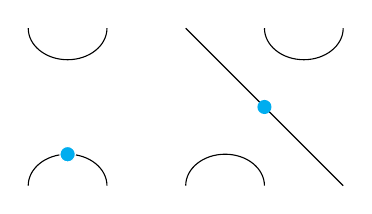
\begin{tikzpicture}
\fivebox{0};
\draw (1,0) arc (-180:0:0.5 and 0.4);
\draw (4,0) arc (-180:0:0.5 and 0.4);
\draw (3,0) -- (5,-2)
	node[fill=cyan,  pos=0.5, shape=circle, inner sep=1.8pt, minimum size=2pt]{};
\draw (1,-2)  arc (180:0:0.5 and 0.4) ;
\draw (3,-2)  arc (180:0:0.5 and 0.4) ;
\draw[fill=cyan, draw=white]{(1.5,-1.6) circle (2.8pt)};
\end{tikzpicture}
\caption{Type II}
\label{fig:type2diag}
\end{subfigure}
\caption{$D$-admissible diagrams.}
\label{fig:diag}
\end{figure}


\begin{example}
\rm Figure \ref{fig:diag} shows an example of a type I diagram and a type II diagram.
\end{example}

%\begin{remark}
%\rm Type I $D$-admissible diagrams have at least one non-propagating edge.
%\end{remark}

\begin{proposition} \label{isomorphic}
{\rm (Green,~\cite{Green1998a})} In type $D_{n}$, the number of $D$-admissible diagrams of type~I is $C(n)-1$, and the number of type~II is $\frac{1}{2}{2n\choose n}$. Therefore, the total number of $D-$admissible diagrams is $\(\frac{n+3}{2}\)C(n)-1$.
 \qed %cite chapter 2 for definition of C(n)
\end{proposition}

\begin{proposition}
{\rm (Green,~\cite{Green1998a})}
The $D$-admissible diagrams form a basis of $\DTL(D_{n})$ and thus $\dim\left(\DTL(D_{n})\right)=\(\frac{n+3}{2}\)C(n)-1$.
\qed
\end{proposition}

\begin{theorem}
{\rm (Green,~\cite{Green1998a})}
As $\Z[\delta]$-algebras, the diagram algebra, $\DTL(D_{n})$, is isomorphic to $\TL(D_{n})$ under $\theta$ as defined in Proposition~\ref{prop:surjective homomorphism}. Moreover, the monomial basis for $\TL(D_{n})$ is in natural bijection with the $D$-admissible diagrams.
\qed
\end{theorem}

%\begin{theorem}
%{\rm (Green,~\cite{Green1998a})} The algebra $\TL (D_{n})$ arises from $\DTL(D_{n})$ as an algebra of diagrams via generators $b_{\overline{1}},b_{1},b_{2},\ldots ,b_{n-1}$ and relations shown in Figure~\ref{fig:relations}. There is a basis for $\TL (D_{n})$ which is in natural bijection with elements of $\DTL(D_{n})$ which have at most one decoration on each edge or loop and which satisfy one of two mutually exclusive conditions of  D-admissible diagrams.
%\qed
%\end{theorem}

%\begin{lemma} \label{isomorphic}
%{\rm (Green,~\cite{Green1998a})} In type $D_{n}$, the number of $D$-admissible diagrams of type~I is $C(n)-1$, and the number of type~II is $\frac{1}{2}\(2n\atop n\)$. Therefore, the total number of $D-$admissible diagrams is $\(\frac{n+3}{2}\)C(n)-1$, which is the dimension of $\TL(D_n)$. \qed %cite chapter 2 for definition of C(n)
%\end{lemma}

%It follows from Lemma~\ref{isomorphic} that the diagram algebra,$\DTL(D_{n})$, is isomorphic to $\TL(D_{n})$. 
\end{section}


%Need thm about D-admissibles being a basis




